%Template prepared by grzegorz ha\l aj for second AMaMeF conference, 17 Oct 2006


\documentclass[12pt]{article}


\usepackage[top=1.5in, bottom=1.5in, left=1in, right=1in]{geometry}


\usepackage{calc}
\usepackage{color}
\usepackage{amsfonts}
\usepackage{latexsym}
\usepackage{placeins}
\ifx\pdftexversion\undefined
  \usepackage[dvips]{graphicx}
\else
  \usepackage[pdftex]{graphicx}
\fi
\usepackage{amssymb}
\usepackage{authblk}
\usepackage{amsmath}
\usepackage[cp1250]{inputenc}
\usepackage[OT4]{fontenc}

\addtolength{\voffset}{-3.5cm} \addtolength{\textheight}{4cm}

\renewcommand\Authfont{\scshape\small}
\renewcommand\Affilfont{\itshape\small}
\setlength{\affilsep}{1em}

\newcommand{\smalllineskip}{\baselineskip=15pt}
\newcommand{\keywords}[1]{{\footnotesize\hspace{0.68cm}{\textit{Keywords}: }#1\par
  \vskip.7\baselineskip}}
\renewenvironment{abstract}[0]{\small\rm
        \begin{center}ABSTRACT
        \\ \vspace{8pt}
        \begin{minipage}{5.2in}\smalllineskip
        \hspace{1pc}}{\end{minipage}\end{center}\vspace{-1pt}}
\newcommand{\emailaddress}[1]{\newline{\sf#1}}

\let\LaTeXtitle\title
\renewcommand{\title}[1]{\LaTeXtitle{\large\textsf{\textbf{#1}}}}

%%%TITLE
\title{Data-driven Koopman theory revisited}
\date{}

%%AFFILIATIONS
\author[1]{Jean-Christophe Loiseau}
\affil[1]{Arts \& M�tiers Institute of Technology, Paris, France \emailaddress{jean-christophe.loiseau@ensam.eu}}

%%DOCUMENT
\begin{document}
\maketitle

%%PLEASE PUT YOUR ABSTRACT HERE

Starting with the seminal works of Clancy Rowley (\emph{J. Fluid Mech.}, 2009) and Peter Schmid (\emph{J. Fluid Mech.}, 2010), approximating the Koopman and Perron-Frobenius operators from data has attracted a lot of attention in the past decade.
These data-driven formalisms suggest new ways of obtaining low-order models from experimentally accessible measurements, most notably for control purposes.
Loiseau \& Brunton (in preparation) have recently realized that \emph{Dynamic Mode Decomposition} (DMD), the most widespread algorithm for data-driven approximation of the Koopman operator, is a special instance of a more general optimization problem, paving the way for a better understanding of the properties of these data-driven models.

After having introduced this general optimization problem and its closed-form solution, I will show the equivalence between DMD and classical linear system identification techniques (e.g. ERA, N4SID, etc).
I will then illustrate how to combine these data-driven models with \emph{Kalman filtering} and \emph{Model Predictive Control} to manipulate increasingly complex nonlinear dynamical systems.
If time permits, some elements pertaining to near-optimal sensor selection will also be discussed.

\vfill

\begin{figure}[h]
  \centering
  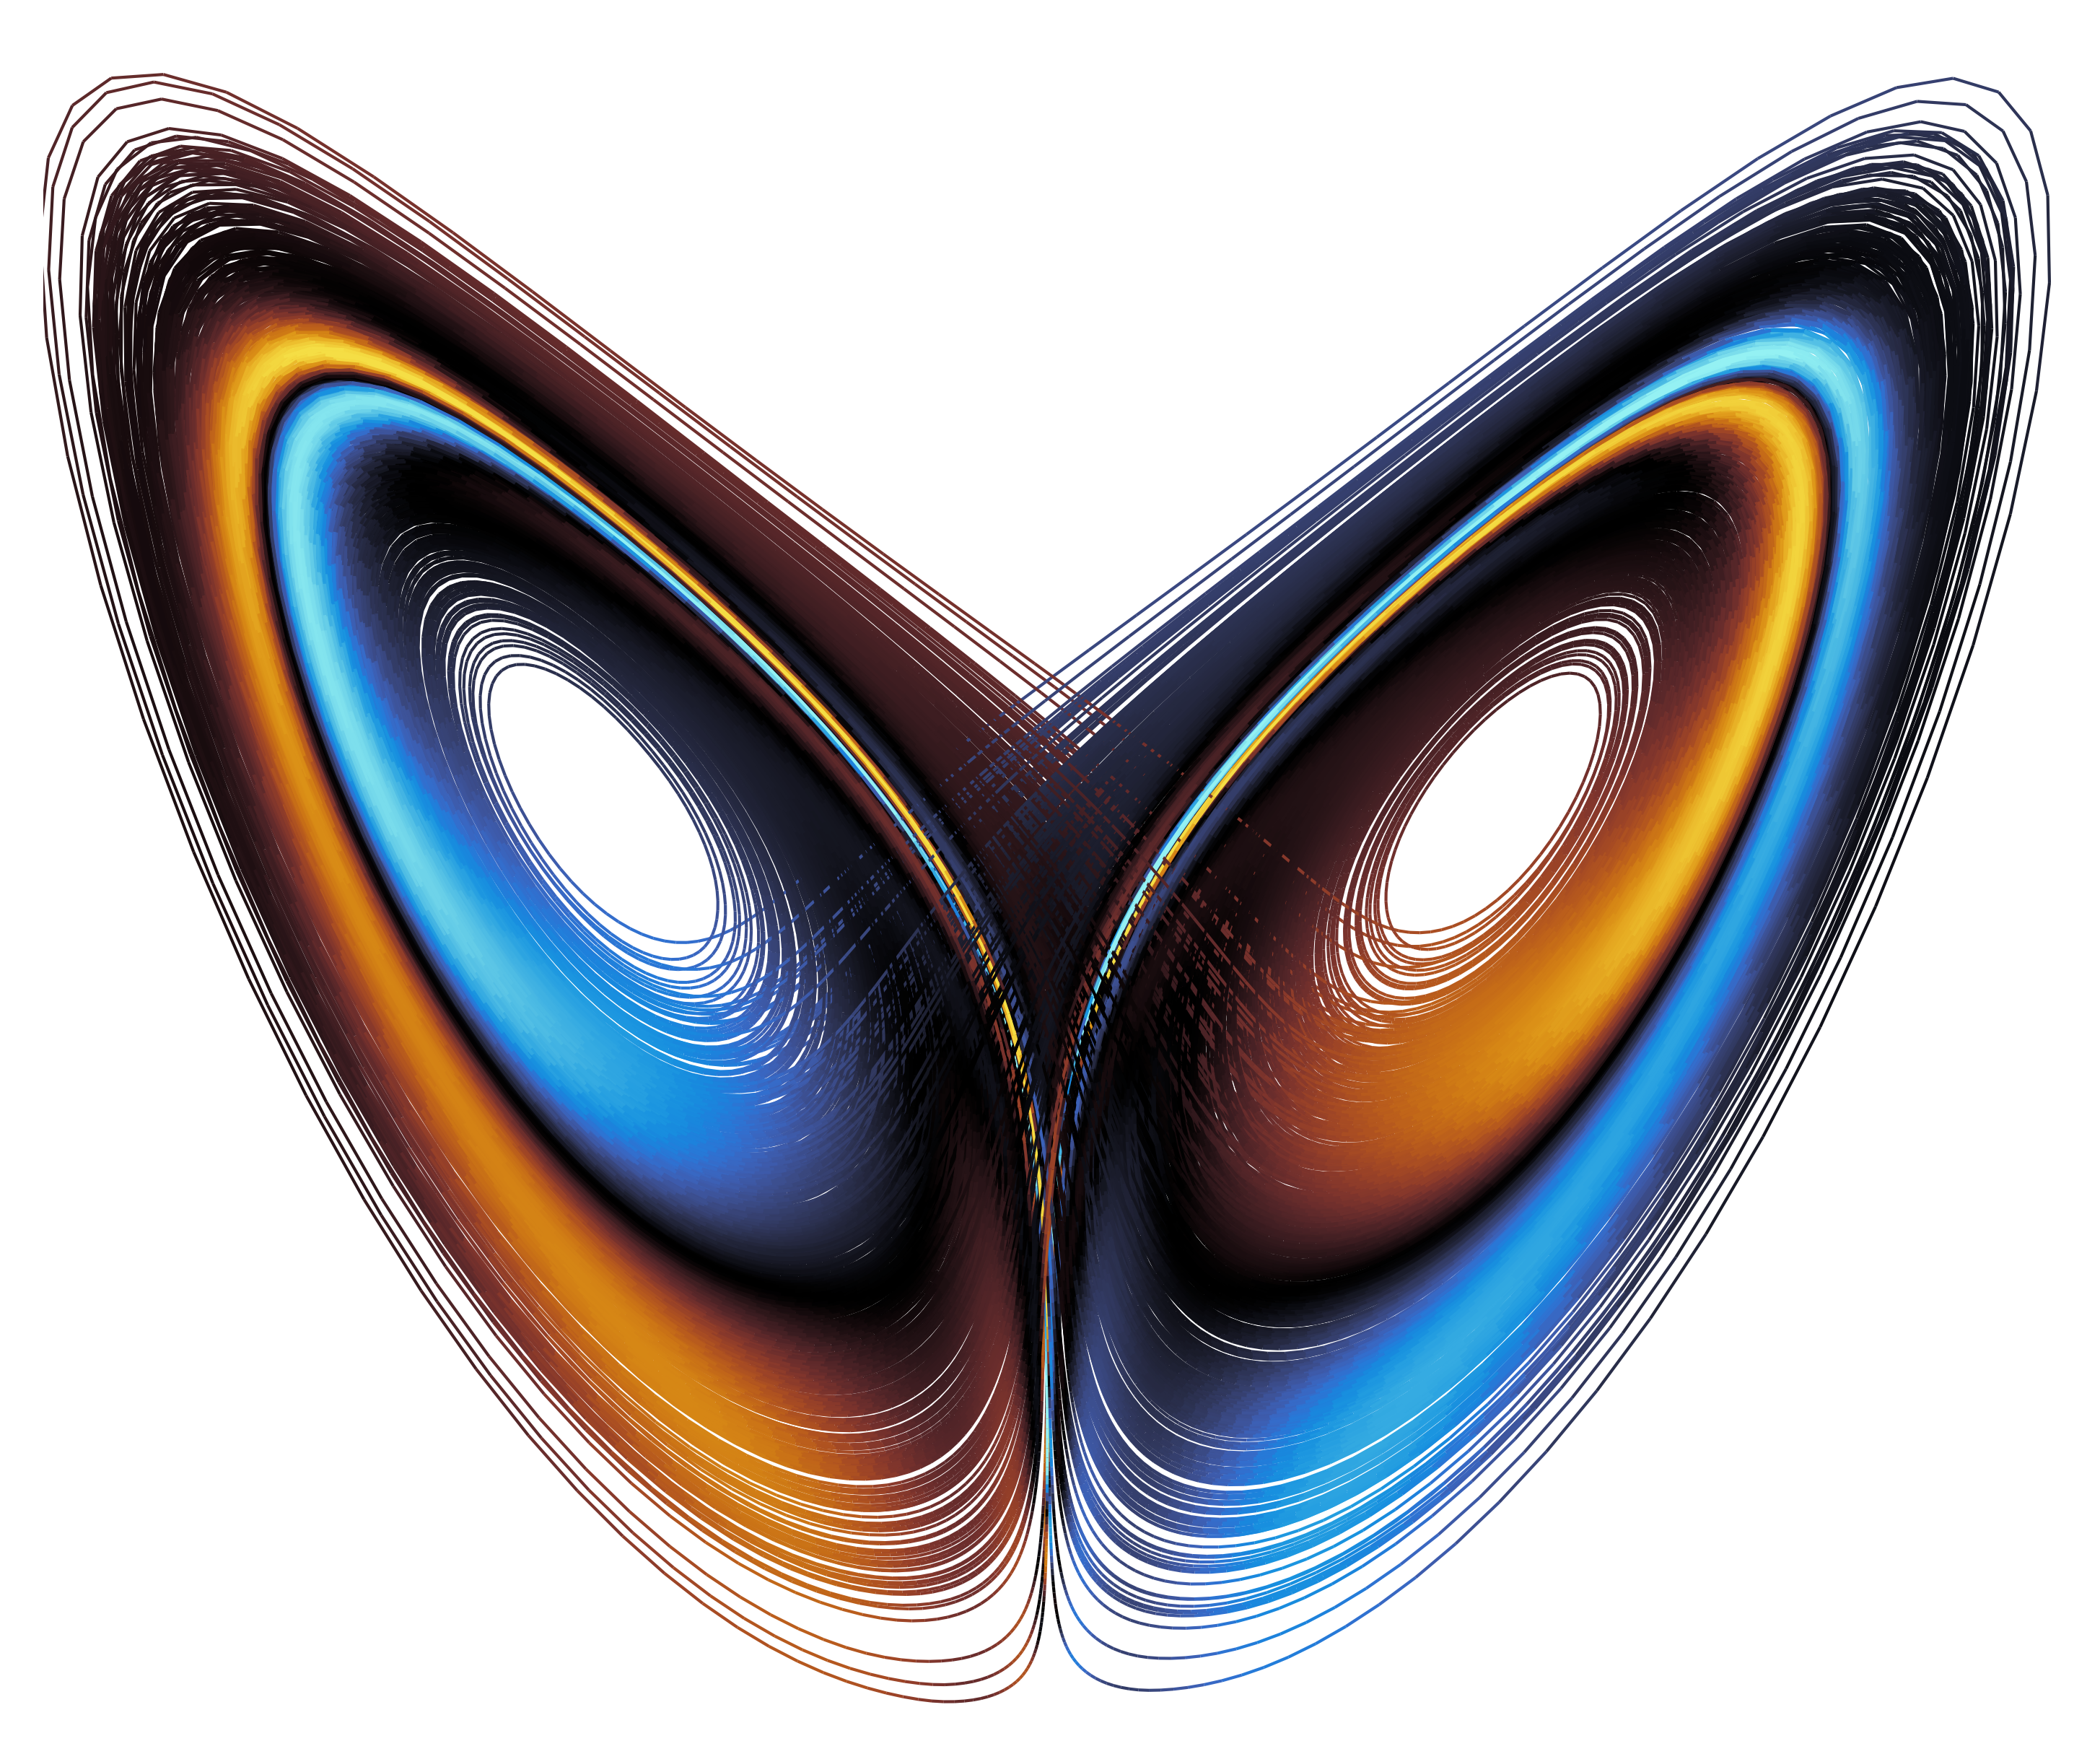
\includegraphics[width=.33\textwidth]{lorenz_singular_function}
  \caption{
    Data-driven approximation of the leading Koopman singular function for the choatic Lorenz 1963 model.
    The observable considered consists in time-delayed measurements of the state variable $x(t)$.
    Blue and orange regions nicely approximate the almost-invariant sets of the dynamics.
  }
\end{figure}


% \begin{thebibliography}{99}
% \small
% \bibitem[1]{kowalski} Kowalski J. \textit{On inexistance of strange
% options}, Medieval Markets, Varsovia, pp. 1--100, 1478.

% \bibitem[2]{smith} Smith J., \textit{How a strange portfolio could look
% like?} Acta Mathematicae --- Medius Aevus, Krak�w, pp. 12012--12312,
% 1221.
% \end{thebibliography}
\end{document}
